%\documentclass[bsc,frontabs,twoside,singlespacing,parskip]{infthesis}
\documentclass[12pt,a4paper,notitlepage]{article}

\title{Exploiting Mobile Entities for Urban Air Quality Monitoring}
\author{Dale Myers}
\date{January 27, 2014}


%\course{Master of Informatics}
%\project{{\bf MInf Project (Phase 2) Report}}


\usepackage{tabularx}
\usepackage{float}
\usepackage{url}
\usepackage{verbatim}
\usepackage{fixltx2e}
\usepackage{graphicx}
\usepackage{parskip}
\usepackage{hyperref}
\usepackage{mhchem}
\usepackage{todonotes}
%\usepackage{minted}
\usepackage{upgreek}
\usepackage{comment}
\usepackage{fullpage}
\usepackage{pdflscape}
\usepackage[toc,page]{appendix}
\usepackage{footnote}
%\usepackage[a4paper]{geometry}
\usepackage{enumitem}


\newcommand{\mahesh}[1]{\todo[inline,color=green!40]{#1}}
\newcommand{\idea}[1]{\todo[inline,color=blue!40]{#1}}
\newcommand{\tdi}[1]{\todo[inline]{#1}}

%This removes the chapter numbering since we don't have chapters
\renewcommand*\thesection{\arabic{section}}

\begin{document}

\maketitle
\thispagestyle{empty}
\newpage

\tableofcontents
\thispagestyle{empty}
%\todototoc
%\listoftodos

\newpage

\setcounter{page}{1}



\section{Introduction}

Over the first year of the project many different aspects of monitoring the air quality around Edinburgh were explored. These included producing a definitive definition of ``air quality'', researching the hardware required to build a cheap air quality sensor, and solving the best ways to represent this data in order to make it as useful as possible. The project was based on the fact that physical sensors would be created and placed on buses owned by the \emph{Lothian Buses} company. However, due to a previous commitment of theirs with another group in the university, this plan proved to be impossible. With a lack of a physical model to create and test the only solution that remained was simulation. The previous semester has been spent creating and running simulations of buses moving around the city of Edinburgh, recording and transmitting data, and logging their results. A further part of the previous semester has been spent designing an outline for the final report for this project. At this point in time the design looks similar to the following:

\begin{enumerate}[itemsep=0mm]
	\item Introduction
		\begin{enumerate}[itemsep=-2mm]
			\item Problem Statement
			\item Commercial Solutions
			\item Current Infrastructure
		\end{enumerate}
	\item Research
		\begin{enumerate}[itemsep=-2mm]
			\item Air Quality
			\item Data Representation
			\item Geostatistical Modelling
			\item Sensor Creation
		\end{enumerate}
	\item Simulation
		\begin{enumerate}[itemsep=-2mm]
			\item Simulators
			\item Creation
			\item Optimisation
			\item Results
			\item Conclusion
		\end{enumerate}
	\item Data Validation
		\begin{enumerate}[itemsep=-2mm]
			\item Ideas
			\item Statistical Methods
			\item Implementation
			\item Results
			\item Conclusion
		\end{enumerate}
	\item Conclusions
\end{enumerate}

\section{Simulation}

In order for the results of this project to have any significance or meaning, a reliable simulator must be used. While it is possible that one could emulate network connectivity using a vehicle simulator, it would provide results which would only be a very rough approximation to reality. Instead, a better approach is to use a network simulator which already supports vehicle motion, or supports adding this to it. 

\subsection{ns-3}
When it was decided that a simulator should be used, ns-3 was the first simulator introduced to the project by Dr. M. Marina due to it's recognition of being powerful and realistic. ns-3 is a very popular network simulator, with a lively community based around it, relatively speaking. Created as a successor to ns-2, which was created by \emph{DARPA} originally, the ns-3 simulator has not only been used in many different academic papers with great results ~\cite{highperformancesimulatorofadhocnetworks}, but when compared to other popular simulators such as ns-2, Omnet++ and JiST, it demonstrated the best overall performance.~\cite{networksimulatorcomparison}. Rather than using a scripting language to create a simulation, ns-3 is instead a framework which can be used in any application. Most of these simulations tend to be written in C++ but support for Python also exists. 

The use of ns-3 for the simulator in this project was attempted for almost 4 weeks, but given that in that time no substantial progress had been made towards achieving the goals of the project, the use had to be carefully evaluated and alternatives explored. 

\subsection{Omnet++}
When ns-3 proved to be difficult to work with for beginners in the area of network simulation, the suggestion of using Omnet++ was put forward by Dr. D.K. Arvind and Dr. S. Viglas. Omnet++, which stands for \emph{Objective Modular Network Testbed in C++}, is not a network simulator in the same way that ns-3 is. It is, instead, a framework which uses discrete events as its basis. Simulations for Omnet++ are also written in C++, but follow a different approach. The simulator uses a collection of modules which follows a strict object oriented model. New modules can be created by sub-classing others, or simply connecting them. With respect to these modules, there are many different collections of these modules, known as ``models''. Many models exist for Omnet++ including, but not limited to, Castilla, INET and MiXiM, with the latter two being of particular interest. In terms of performance and accuracy, Omnet++ rivals ns-3~\cite{networksimulatorcomparison}.

MiXiM is used in Omnet++ for creating wireless networks with a particular focus on the lower layers of the network stack. The models provided in the MiXiM framework are extremely detailed and include radio wave propagation, interference estimation, radio transceiver power consumption and wireless MAC protocols~\cite{miximvision}. MiXiM has no support for the upper network layers and if you need these then you need to rely on another model such as INET, or create your own. The features in MiXiM are extremely advanced and it was therefore decided that it is more complex than required for this application. While it wouldn't change the results by using MiXiM, it would slow the simulation down considerably.

INET is very closely related to Omnet++ in that it is rare to use Omnet++ without using INET. INET provides models for the internet stack, as well as wired and wireless link layer protocols. It also contains many different application layer models, mainly for demonstration purposes.  

\subsection{Creating the Simulation}

The position data provided by Lothian Buses had the positions of 145 different buses across a 24 hour period. This means that we have to be able to simulate 145 buses moving around and connecting to various access points. As for the access points, a PhD student of Dr. Marina, Arsham Farshad, provided a list of open wifi access points around the city. In total there were over 2000 access points and as can be seen in the graph in figure~\ref{fig:aptimes} this would take a hugely long time to simulate. Instead the decision was made to limit the number of access points to 50. Even so, certain simulations would have taken many days to simulate a single day of events. 

\begin{figure}[H]
    \begin{center}
        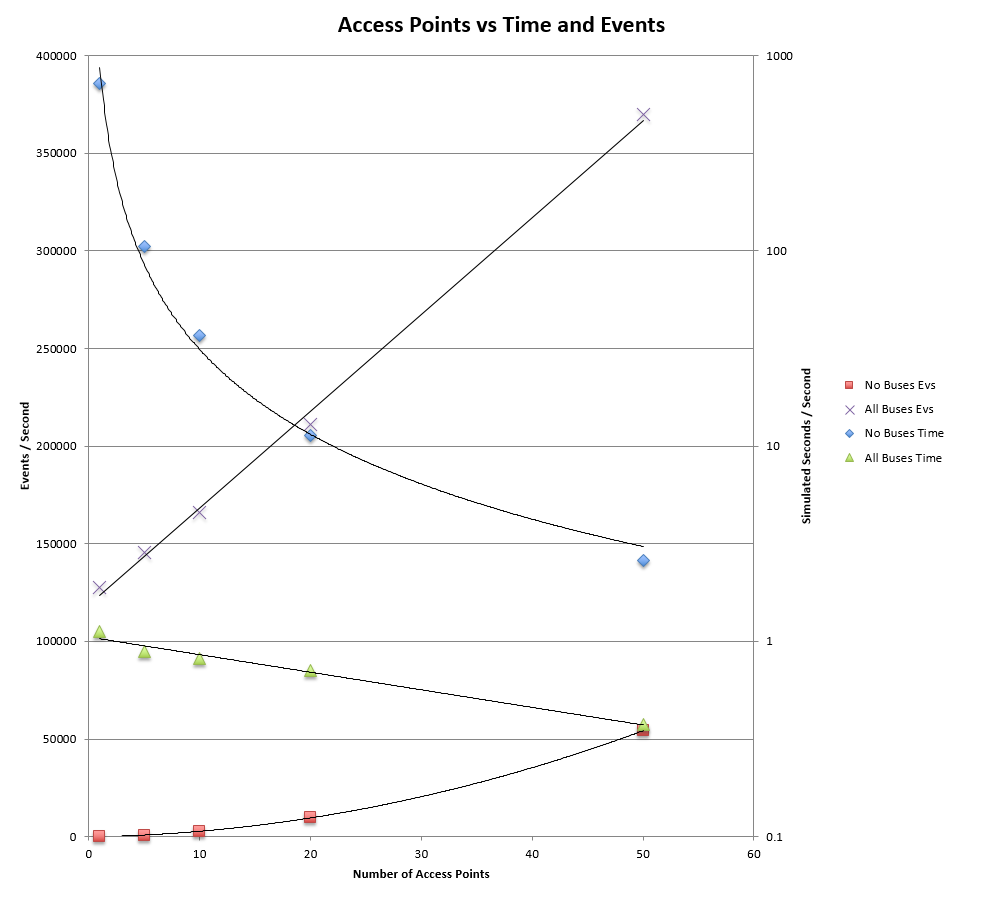
\includegraphics[width=\textwidth]{../images/AP_vs_Time_and_Events.png}
        \caption{An example of how simulation time and events change with the number of access points.}
        \label{fig:aptimes}
    \end{center}
\end{figure}


\subsubsection{Bus Mobility}

The data provided by Lothian Buses was provided in an interesting format. Every 30 seconds there was a list of the last reported positions of the buses. There was a huge variation between times that the GPS co-ordinates were reported back and the accuracy of the measurements with some buses reported as being in Wales. The first step in making the data usable was to get it into a consistent format. This was done by creating a processing script which removed duplicate data points, converted the co-ordinates from Eastings and Northings into Latitude and Longitude, and added the timestamped points into a database. 

After getting this information into the database we needed to find out which buses are on which routes in order to deal with the opportunistic forwarding at a later point. This classification had to be done manually which took a considerable amount of time. With the classification in place the final step was interpolation. We only had readings of roughly every 30 seconds, which would not be enough to reliably check interactions between buses. In order to combat this, interpolation was used across the data set in order to have positions every single second. An example of how this data would look (with only 1 in 10 points shown) can be seen here: \url{http://myers.io/map.php?busId=726&startTime=2013-08-09+19%3A19%3A00&endTime=2013-08-09+19%3A40%3A00&submit=Interpolated}

A final optimisation which was necessary was a small study into databases so that the simulation could access the data as efficiently and quickly as possible. With the current setup the data was stored on a virtual machine running on a home server. This machine was not fast by most standards, nor is the connection able to rival a hosting providers. As such, with over twelve million data points required per simulation, the decision was made to move the data into a local database for faster access. This involved exporting the database to an sqlite database. This was achieved with a script created by the \emph{GitHub} user \emph{esperlu}~\cite{mysql2sqlite}, producing a 1 GB file which, by modern standards, is very manageable. 

\subsubsection{Access Point Positions}

As previously mentioned, there would be no more than 50 access points due to processing time requirements. This relatively small number meant that instead of wasting processing power and time by reading in from an external source, the access point positions could simply be hard coded into the simulation, and indeed this is encouraged for smaller data sets. By using the data provided by Arsham Farshad, I was able to find from a list of 2945 access points, those with the strongest signals. The measure of signal strength used received signal strength indication which uses arbitrary units. In order to have a reasonable list of access points I chose a threshold which would give roughly 100 access points to choose from. The final number to choose from was 82. For different runs of the simulation with $n$ access points, $n$ unique positions were randomly chosen from this list. 

\subsection{Optimisations}

As can be seen in figure~\ref{fig:aptimes}, as we increase the number of access points, and indeed buses, the simulation time increases. By experimentation, with all 145 buses and 50 access points, running on a reasonable laptop computer, the entire simulation would take around 4 days to run. In order to combat this each experiment was run for 10,000 simulated seconds (almost 3 hours), instead of the full 24 hours. With experimentation with 5 different access point numbers, 4 different queue sizes and 5 different runs, this still would take $5 * 4 * 5 * 6 = 600$ hours, which is 25 days. In order to run experiments in any meaningful time things would have to change. 

\subsubsection{MPI}

The first mode of optimisation visited was using MPI, which stands for \emph{Message Passing Interface}. Omnet++ has support for MPI out of the box~\cite{omnetmpi} and so it seemed like a good place to start. After looking into the topic it seemed that MPI would probably not speed up the simulation by much if at all. Generally simulations which are suited to this are networks which have a partition between them. An example of this would be two networks connected by a single connection. Each network could be simulated on a different processor or machine and only messages between the two networks need to use MPI. In this projects simulation we have many different components with no clear partition. Access points are always talking to different buses and there would be no way of partitioning in an effective manner without manually comparing positions and routes of buses with access points and placing these access points and buses on the same processor or machine. When experimenting with MPI on 2, 4 and 8 processors, the simulation took longer and longer than it did with a single processor. Review of the logs showed that most of the time was spent passing messages between processors. Using multiple machines would only make things slower due to the network connection. It seems reasonable however that if each access point and bus could be placed on a seperate machine then we may get a small speed boost, however this would require almost 200 machines and is therefore not feasible. 

\subsubsection{Parallel Execution}

With the failure of MPI, an alternative was needed. Further research and recording showed that the simulation process was single threaded and therefore bound to a single processor. On a dual core processor, it was estimated that we could run two simulations at almost the same speed as a single simulation on the same machine. Testing this theory revealed that simulations took roughly twice as long when doing this. No reason could be found for this, but it was suggested that interaction with other components such as the file system when logging data was causing the problems with two simulations running, as both had to wait for the other often. 

The solution to this was to run it on different machines. If we were to put each run on a different machine then we could decrease our run time by a factor of 5, bringing the total time down to roughly 120 hours, which is 5 days. Unfortunately 5 machines were not available that could run for 5 days to get these results  and an alternative was found. \emph{Digital Ocean}~\cite{digitalocean} are a cloud hosting company with relatively low cost. The parallel execution experiments revealed that at least two cores were required for running a simulation effectively and so I created 5 virtual servers using Digital Ocean which had 2 cores at the cheapest cost. The times of execution varied depending on the physical server they were on, but most simulations ended up taking a similar time to the laptop they were originally tested on, at around 5 days in total. This has allowed two different experiments to be created which have evaluated 4 different parameters in turn, for a relatively low cost of \$40.

\section{Current Results}

The completion of the first stage of the simulation allowed experiments to be run. The experiments were designed to provide information about how varying certain parameters altered the packet delivery ratio and latency. These parameters were the queue size for the readings, the number of access points, the power level of the radios and different propagation models. This section aims to give a brief overview of the current results.

\subsection{Queue Size}

\begin{figure}[H]
    \begin{center}
        \makebox[\textwidth][c]{
            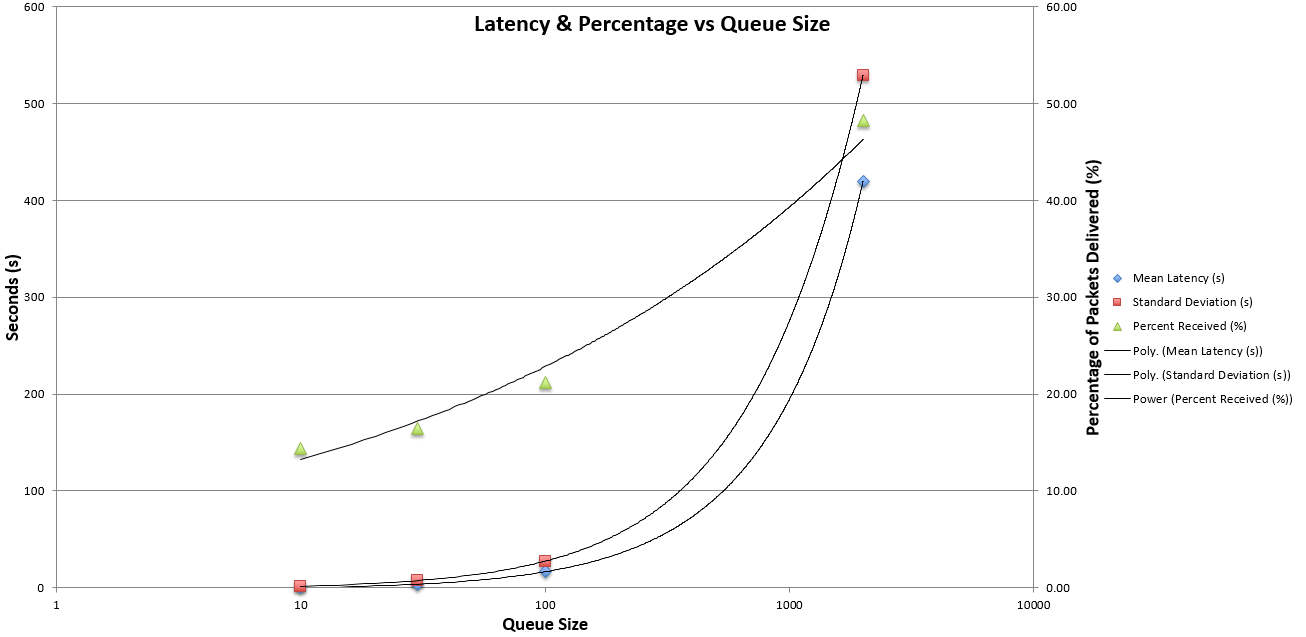
\includegraphics[width=\textwidth]{../images/Latency_Percentage_vs_Queue_Size_Log.png}
        }
        \caption{A graph showing how latency and percentage of packets received changes with the queue size of the sensors.}
        \label{fig:queuesize}
    \end{center}
\end{figure}

Figure~\ref{fig:queuesize} is the result of running 5 different simulations with different access points chosen randomly. The queue size on the buses was varied between 10, 30, 100 and 2000. The effects of changing the queue size area clear. As the queue size increases, so does the latency of the packets being delivered, but importantly, it also increases the packet delivery rate. The reason for this is simple, as we have a larger queue size, we can hold onto more packets, and therefore deliver more. The penalty is that the packets we hold on to could be in the buffer for up to $n$ seconds, where $n$ is the size of the buffer, assuming there is a reading once per second.

\subsection{Model}

\begin{figure}[H]
    \begin{center}
        \makebox[\textwidth][c]{
            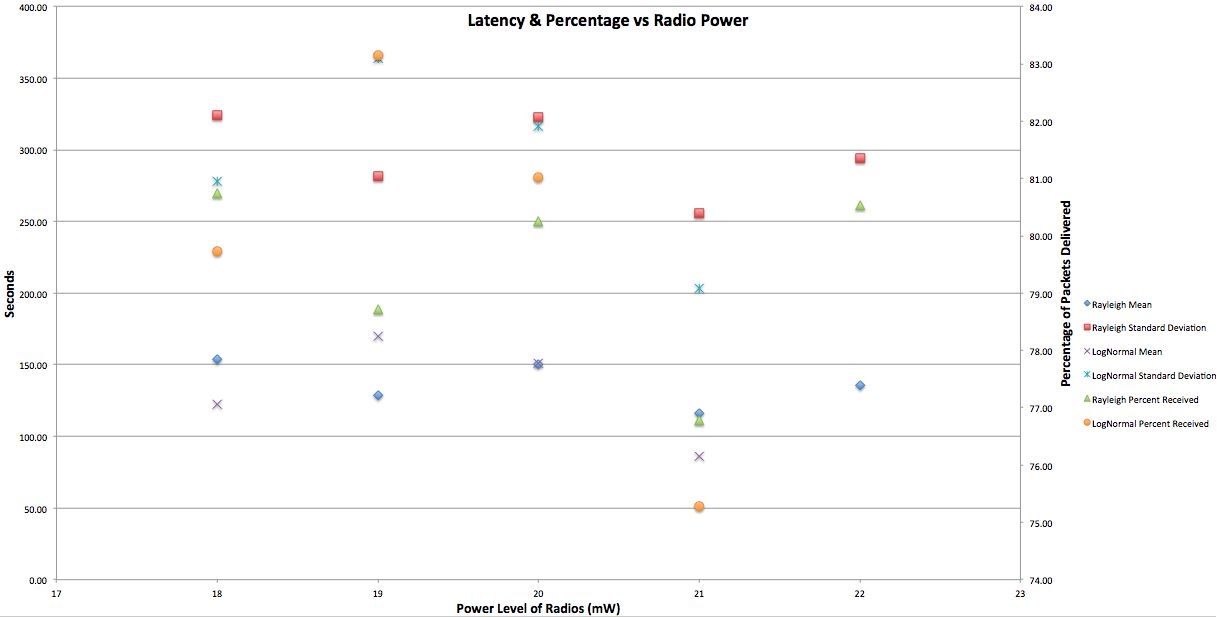
\includegraphics[width=\textwidth]{../images/Latency_Percentage_vs_Radio_Power.png}
        }
        \caption{A graph showing how latency and percentage of packets received changes with the power of the radios for two different propagation models.}
        \label{fig:radiopower}
    \end{center}
\end{figure}


With the changes to the propagation model, it is a little more difficult to see any clear pattern. By comparing the means of the Rayleigh model and the Log Normal Shadowing model, there is very little evidence to show a clear difference. Comparing the standard deviations reveals nothing more, however the readings of mean and standard deviation are consistent between models which suggests that is is not merely chance that there is no clear difference. When we look at the percentage of packets received it once again follows the same pattern. 

\subsection{Transmitter Power}
 
With respect to transmitter power, this is the only metric where we can glean any information. The most information we can see is that at different powers, the different models react differently. At 19mW the Log Normal Shadowing model outperforms the Rayleigh model, however at 20mW they are comparible, and at 18mW and 21mW the Rayleigh model is the superior one. The reasons for this at the current time are unclear. However, due to bugs within Omnet++ the simulations did not run for as long as intended, averaging around 1,500-2,000 seconds rather than the intended 10,000. It shall be determined if the shorter run time is the cause of this. 

\section{Future Work}

With regards to future work there are two parts remaining. The first is a change to the simulation to add in opportunistic forwarding. This will add secondary radios to each of the buses and pass data between buses should it be advantageous to the delivery of the data. The second part is more significant and it is evaluating the data I have using statistical modelling to verify if the data returned by buses would be of any use should this system become a physical reality. 

\subsection{Opportunistic Forwarding}

Opportunistic forwarding is the system which stands to bring the most efficiency to the current model. When looking at hardware which could feasible be used in such a sensor should it be made, a reasonable candidate, due to it's cost, power and use in similar projects~\cite{arduinoproj1}~\cite{arduinoproj2}~\cite{arduinoproj3}, for the processing module would be an Arduino Uno. An Arduino Uno could deal with our maximum tested queue size of 2000 packets, assuming an 16 byte packet, but not much more~\cite{arduinounospecs}. Due to these size constraints, we need a way of dealing with storage space. One possible solution is to simply find a way to add more flash memory, however with this method we run into problems with the capacity of that storage. It is entirely possible that there are buses on more rural routes which rarely see open access wifi points. A much better solution to adding storage is to add a second radio to the sensors. This second radio could be used to form an ad-hoc network with any nearby buses. The buses will have statistics recorded of how often they see access points and can therefore estimate when they will next encounter one and for how long they will be in contact with it. By performing these simple calculations the buses can decide if it is best for one to send some of its data to the other or not. 


\begin{figure}[H]
    \begin{center}
        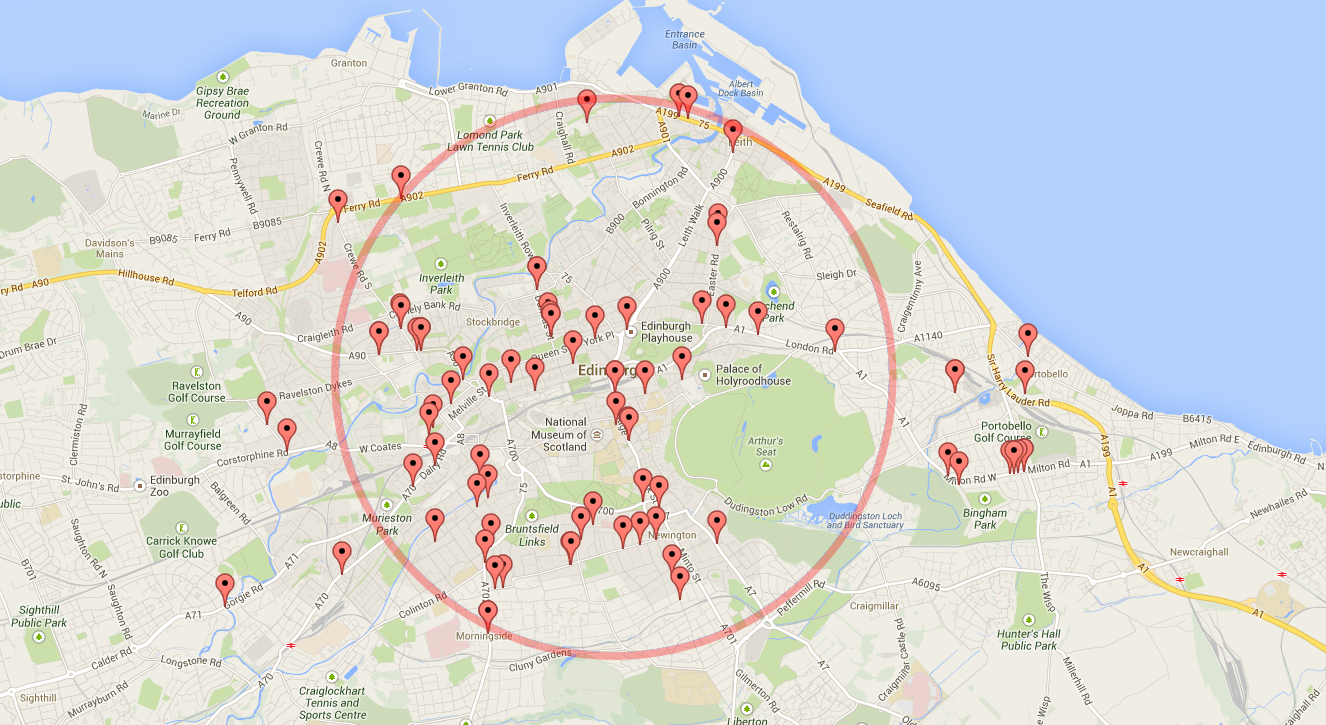
\includegraphics[width=\textwidth]{../images/APMap.png}
        \caption{A map of the 89 access points used in the simulations. Image uses \emph{Google Maps}.}
        \label{fig:apmap}
    \end{center}
\end{figure}

\begin{figure}[H]
    \begin{center}
        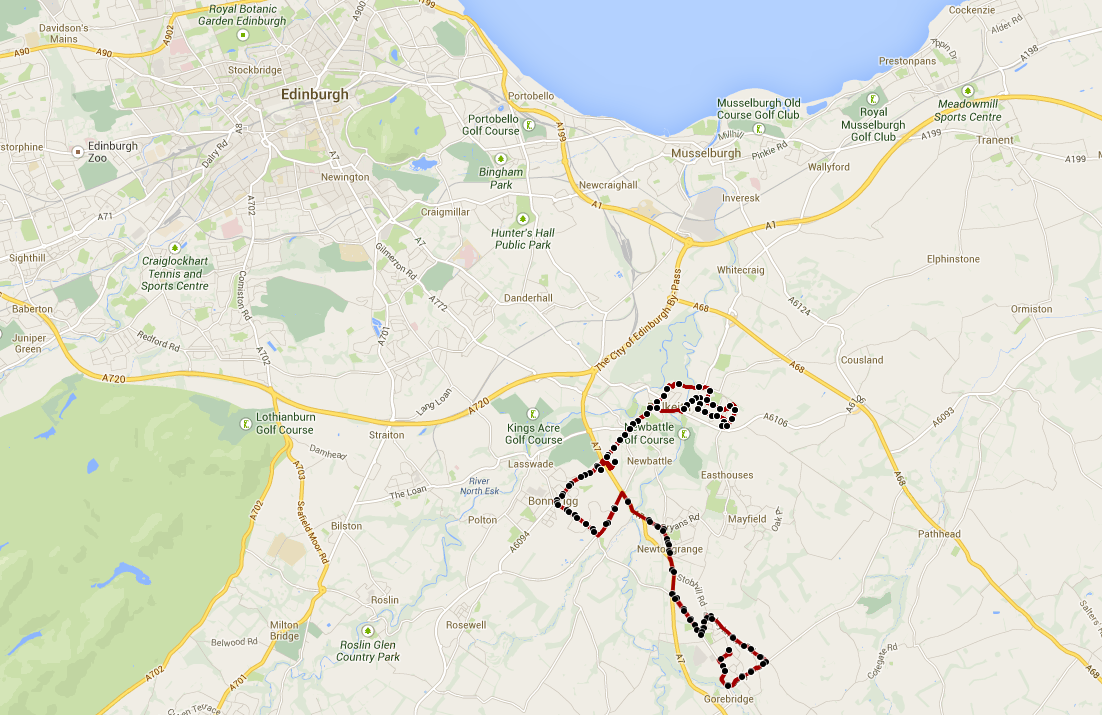
\includegraphics[width=\textwidth]{../images/Route39.png}
        \caption{A map of the Lothian Bus route 39. Image uses \emph{Google Maps}.}
        \label{fig:route39}
    \end{center}
\end{figure}


In figure~\ref{fig:apmap} we can see that the access points which are used in the simulation are all around the city centre. Some routes run the risk of buses not coming into contact with any access points, or not coming into contact with them for long enough. However, they will always pass other buses en route, which could be enough to pass on the rest of the data which otherwise would be lost due to storage requirements. An example of this is route 39. Figure~\ref{fig:route39} shows the route of the 39. This route is entirely outside the bypass, and out with the range of access points recorder. In a simulation, this bus would never return any data. However, if we look at the same image with the route of the number 40 added in figure~\ref{fig:route3940} then we can see that the 40 is much more likely to pass by access points due to its trip through the much more densely populated areas of Musselburgh and Portobello. These two routes converge for 1.8 miles and according to the bus timetables for these routes, the 39 takes roughly 14 minutes to traverse this length, and the 40 takes around 12 minutes. With the time between each 39 being an hour (therefore half an hour if you take both directions into account), and each 40 being half an hour (therefore 15 minutes), it is likely that in most cases, a 39 will encounter at 40 at some point along the route, which shows that the idea is viable, at least for this situation. By increasing the rate at which a bus can offload packets, we can decrease the queue size and increase the packet size, allowing us to measure more data. 
 
\begin{figure}[H]
    \begin{center}
        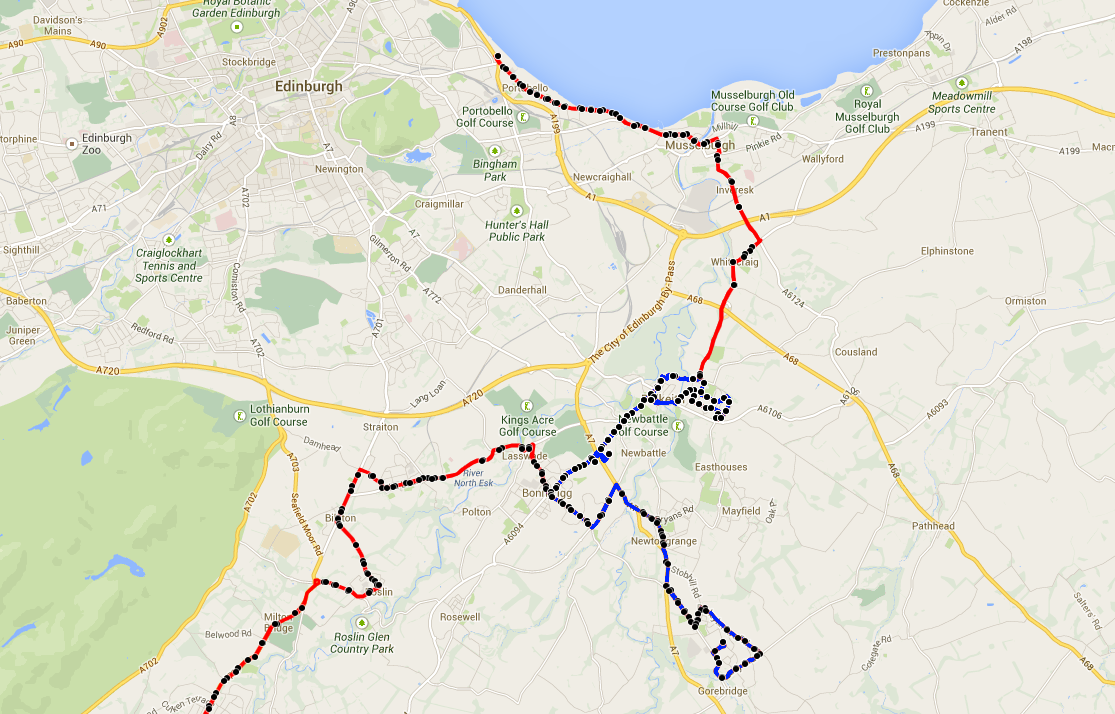
\includegraphics[width=\textwidth]{../images/Route3940.png}
        \caption{A map of the Lothian Bus routes 39 and 40. Image uses \emph{Google Maps}.}
        \label{fig:route3940}
    \end{center}
\end{figure}


\subsection{Data Evaluation}

The final part of the project is evaluating whether the implementation would provide useful data or not. A similar project is currently running in Zurich. The OpenSense~\cite{opensensezurich} project places sensors on trams and is designed to provide data to the general public with minimal cost. The project uses cheap hardware and accurate measurement stations for calibration. If we look at their maps of information we can see that the readings they provide are only along the tram routes. In order for the data that we would potentially collect, should the project be physically realised, to be useful we would have to be able to accurately predict what the concentrations of chemicals are in areas where we do not have sensor readings. 

\begin{figure}[H]
    \begin{center}
        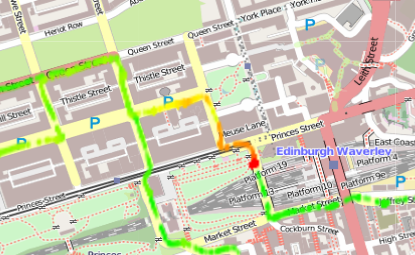
\includegraphics[width=\textwidth]{../images/StationaryPollutantBuildUp.png}
        \caption{A map of air pollution around Edinburgh city centre. Image uses \emph{Open Street Map}.}
        \label{fig:stationarypollutantbuildup}
    \end{center}
\end{figure}


\begin{figure}[H]
    \begin{center}
        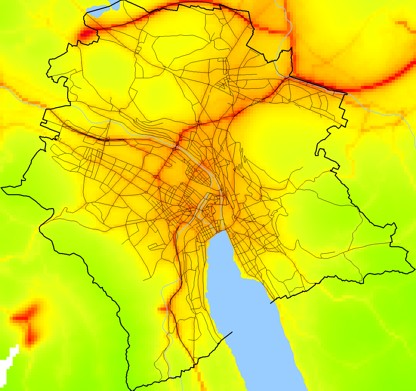
\includegraphics[width=\textwidth]{../images/zurichpm.jpg}
        \caption{A heatmap of particulate matter in Zurich. The higher pollution levels can clearly be seen to follow transport infrastructure.~\cite{opensensezurich}}
        \label{fig:zurichheatmap}
    \end{center}
\end{figure}

When taking air pollution readings a map of concentrations can be generated which looks similar to that of figure~\ref{fig:stationarypollutantbuildup}. These readings are clearly confined to their immediate vicinity and show no information about surrounding areas. If were were to use some statistical method, we could estimate with some degree of certainty what the pollution levels are in areas where there are no recordings. By doing this we could produce a map similar to the one in figure~\ref{fig:zurichheatmap}.


In order to solve this problem and accurately predict the pollution levels, one would need to do multiple PhDs in order to accurately perform and understand this task. Instead, on a simpler level, we will employ existing tools to help us perform this task. By using well known and understood methods, avoiding complex methods such as regression kriging~\cite{regressionkriging}, which are provided in a single tool or package, such as an R or Python library, we will attempt to prove that this data is at least accurate enough to provide a high level overview of pollution across the city. 

In order to validate whether our results are correct or not, we will use the freely available data from the OpenSense project and perform our analysis on this. To measure the effectiveness of our methods we will find locations where static air quality monitoring stations exist and use our motion results to estimate the pollutant levels at this location. We can then compare and contrast our calculated results with the actual results and use this to evaluate our model. 

\addcontentsline{toc}{section}{References}
\bibliographystyle{unsrt}
\bibliography{../references}


\end{document}



